% F1R3Ink — Game Design, version 1
% Build: xelatex f1r3ink-design.tex (twice). Brand fonts are read from ./fonts,
% logos from ./logos (both copied from github.com/F1R3FLY-io/f1r3fly-brand-portal).
\documentclass[11pt,a4paper]{article}

\usepackage[a4paper,top=30mm,bottom=26mm,left=22mm,right=22mm,headsep=10mm,footskip=12mm]{geometry}
\usepackage{fontspec}
\usepackage{xcolor}
\usepackage{graphicx}
\usepackage{tikz}
\usetikzlibrary{arrows.meta,positioning,calc,fit,backgrounds}
\usepackage{titlesec}
\usepackage{fancyhdr}
\usepackage{enumitem}
\usepackage{booktabs}
\usepackage{tabularx}
\usepackage{array}
\usepackage{listings}
\usepackage[most]{tcolorbox}
\usepackage{amsmath,amssymb}
\usepackage[hidelinks]{hyperref}
\usepackage{etoolbox}
\usepackage{microtype}

% ------------------------------------------------------------------ brand
% Colour system of 12 June 2026 (brand kit v1.2). White interior surface for a
% printable technical document: Yellow and Sky appear as rules and fills only,
% never as text, because both fail contrast as text on white.
\definecolor{brandyellow}{HTML}{F3D630}
\definecolor{brandsky}{HTML}{3FA9F5}
\definecolor{brandskydark}{HTML}{00528C}
\definecolor{brandblack}{HTML}{000000}
\definecolor{muted}{HTML}{3F3F3F}
\definecolor{footgray}{HTML}{595959}
\definecolor{codebg}{HTML}{F2F2F2}
\definecolor{rulegray}{HTML}{C5C5C5}

% The default ink palette (D4). Used in figures only.
\definecolor{ink1}{HTML}{E6194B}\definecolor{ink2}{HTML}{F58231}
\definecolor{ink3}{HTML}{FFE119}\definecolor{ink4}{HTML}{BFEF45}
\definecolor{ink5}{HTML}{3CB44B}\definecolor{ink6}{HTML}{42D4F4}
\definecolor{ink7}{HTML}{4363D8}\definecolor{ink8}{HTML}{911EB4}
\definecolor{ink9}{HTML}{F032E6}\definecolor{ink10}{HTML}{FABED4}
\definecolor{ink11}{HTML}{DCBEFF}\definecolor{ink12}{HTML}{9A6324}
\definecolor{ink13}{HTML}{800000}\definecolor{ink14}{HTML}{000075}
\definecolor{ink15}{HTML}{A9A9A9}\definecolor{ink16}{HTML}{FFFFFF}

\setmainfont{SourceSans3}[
  Path=./fonts/, Extension=.ttf,
  UprightFont=*-400, BoldFont=*-700, ItalicFont=*-400,
  ItalicFeatures={FakeSlant=0.18}, BoldItalicFont=*-700, BoldItalicFeatures={FakeSlant=0.18}]
\newfontfamily\spartanbold{LeagueSpartan-Bold}[Path=./fonts/, Extension=.ttf]
\newfontfamily\spartansemi{LeagueSpartan-SemiBold}[Path=./fonts/, Extension=.ttf]
\newfontfamily\spartanreg{LeagueSpartan-Regular}[Path=./fonts/, Extension=.ttf]
\newfontfamily\spartanlight{LeagueSpartan-Light}[Path=./fonts/, Extension=.ttf]
\newfontfamily\sourcelight{SourceSans3-300}[Path=./fonts/, Extension=.ttf]
\setmonofont{DejaVu Sans Mono}[Scale=0.84]
\renewcommand{\sffamily}{\spartanreg}

\newcommand{\caps}[1]{{\addfontfeatures{LetterSpace=12}\MakeUppercase{#1}}}
\newcommand{\gradrule}[1][\linewidth]{%
  \noindent\begin{tikzpicture}\shade[left color=brandyellow,right color=brandsky]
  (0,0) rectangle (#1,0.6pt);\end{tikzpicture}}

\hypersetup{colorlinks=true,linkcolor=brandskydark,urlcolor=brandskydark,citecolor=brandskydark,
  pdftitle={F1R3Ink: Game Design},pdfauthor={F1R3FLY.io}}

\titleformat{\section}{\spartanbold\fontsize{13}{16}\selectfont}
  {\caps{\thesection}\hspace{1em}}{0pt}{\caps}[\vspace{3pt}\gradrule]
\titleformat{\subsection}{\spartansemi\fontsize{10.5}{13}\selectfont}{\thesubsection\hspace{0.8em}}{0pt}{}
\titleformat{\subsubsection}[runin]{\bfseries}{}{0pt}{}[.]
\titlespacing*{\section}{0pt}{20pt}{12pt}
\titlespacing*{\subsection}{0pt}{14pt}{6pt}
\setcounter{secnumdepth}{2}
\setcounter{tocdepth}{2}

\setlength{\parindent}{0pt}
\setlength{\parskip}{6pt}
\linespread{1.08}
\emergencystretch=3em

\pagestyle{fancy}
\fancyhf{}
\renewcommand{\headrulewidth}{0pt}
\fancyhead[L]{\raisebox{-2pt}{
\includegraphics[height=7.5mm]{logos/f1r3fly-io-horizontal-logo-white-background.pdf}}}
\fancyhead[R]{\spartanreg\fontsize{8}{10}\selectfont\color{footgray}\caps{F1R3Ink · Game design · v1}}
\fancyfoot[L]{\spartanbold\fontsize{7.5}{9}\selectfont\color{footgray}\thepage}
\fancyfoot[R]{\spartanbold\fontsize{7.5}{9}\selectfont\color{footgray}\textcopyright{} F1R3FLY INDUSTRIES, 2026. All Rights Reserved \textbar{} 8 October 2026}

\lstdefinelanguage{rholang}{
  morekeywords={new,in,for,contract,match,if,else,bundle,Nil,true,false,not,and,or},
  sensitive=true, morecomment=[l]{//}, morestring=[b]"}
\lstset{basicstyle=\ttfamily\small,backgroundcolor=\color{codebg},frame=leftline,
  rulecolor=\color{brandsky},framerule=1.2pt,framesep=6pt,xleftmargin=8pt,
  breaklines=true,columns=fullflexible,keepspaces=true,showstringspaces=false,
  keywordstyle=\bfseries,commentstyle=\color{muted},aboveskip=8pt,belowskip=8pt}

\newcommand{\code}[1]{\texttt{#1}}
% The body face has no small capitals, so RFC 2119 keywords are set in reduced capitals.
\newcommand{\MUST}{{\fontsize{0.82em}{1em}\selectfont MUST}}
\newcommand{\MUSTNOT}{{\fontsize{0.82em}{1em}\selectfont MUST NOT}}
\newcommand{\SHOULD}{{\fontsize{0.82em}{1em}\selectfont SHOULD}}
\newcommand{\MAY}{{\fontsize{0.82em}{1em}\selectfont MAY}}

\newtcolorbox{decision}[2]{enhanced,breakable,colback=white,colframe=white,
  boxrule=0pt,left=10pt,right=4pt,top=4pt,bottom=4pt,
  borderline west={2.2pt}{0pt}{brandsky},
  fontupper=\small,
  title={\spartanbold\fontsize{8.5}{10}\selectfont\color{brandblack}\caps{Decision #1}\quad
         \spartansemi\normalsize\fontsize{10.5}{12}\selectfont #2},
  coltitle=brandblack,colbacktitle=white,attach title to upper,after title={\par\smallskip}}

\newtcolorbox{finding}[2]{enhanced,breakable,colback=codebg,colframe=codebg,
  boxrule=0pt,left=8pt,right=6pt,top=5pt,bottom=5pt,arc=2pt,
  title={\spartanbold\fontsize{8.5}{10}\selectfont\caps{Finding #1}\quad\spartansemi\fontsize{10.5}{12}\selectfont #2},
  coltitle=brandblack,colbacktitle=codebg,attach title to upper,after title={\par\smallskip},fontupper=\small}

\newcounter{req}
\newcommand{\req}[1]{\refstepcounter{req}\label{#1}\textbf{R\thereq}}

% A stripe in figures: \stripe{y}{colour}{opacity}{half-width}
\newcommand{\stripe}[4]{\fill[#2,opacity=#3,rounded corners=0.6pt] (-#4,#1-0.09) rectangle (#4,#1+0.09);}

\begin{document}

% ================================================================= cover
\begin{titlepage}
\newgeometry{margin=0pt}
\pagecolor{brandblack}\color{white}
\begin{tikzpicture}[remember picture,overlay]
  \node[anchor=north] at ($(current page.north)+(0,-38mm)$)
    {
\includegraphics[width=70mm]{logos/f1r3fly-io-vertical-logo-color-on-dark.pdf}};
  \node[anchor=north west,text width=150mm,text=white] at ($(current page.north west)+(30mm,-150mm)$) {%
    {\spartanbold\fontsize{9}{11}\selectfont\color{brandyellow}\caps{F1R3Games · Game design}}\par\vspace{8mm}
    {\spartanlight\fontsize{40}{44}\selectfont F1R3Ink}\par\vspace{5mm}
    {\sourcelight\fontsize{15}{20}\selectfont Collective emotional intelligence on a F1R3FLY shard}\par\vspace{9mm}
    \begin{tikzpicture}\shade[left color=brandyellow,right color=brandsky] (0,0) rectangle (150mm,0.6pt);\end{tikzpicture}\par\vspace{7mm}
    {\fontsize{10.5}{15}\selectfont Version 1 \quad·\quad 8 October 2026\par
     Conforms to F1R3Node-Rust \code{master@3c7872a} and the F1R3Games Portal at\par
     \code{F1R3Games main@5937e4e}, with F1R3Beat as implemented on \code{f1r3beat@57a3b27}}};
  \node[anchor=south east] at ($(current page.south east)+(-22mm,14mm)$)
    {\spartanbold\fontsize{7.5}{9}\selectfont\color[HTML]{C5C5C5}\textcopyright{} F1R3FLY INDUSTRIES, 2026. All Rights Reserved \textbar{} 8 October 2026};
\end{tikzpicture}
\restoregeometry
\end{titlepage}
\nopagecolor\color{black}

% ================================================================= abstract
\begin{center}
\begin{minipage}{0.9\linewidth}
{\spartanbold\fontsize{8.5}{10}\selectfont\caps{Summary}}\par\smallskip
F1R3Ink is a multiplayer game for collecting a community's emotional perceptions of its
members. It has one move. A player selects another player and \emph{inks} them with a colour
that says how they perceive that person at that moment. No colour has a fixed meaning. Each
inker owns one stripe on each person they ink, and re-inking changes the stripe's colour. A
person's stripes, drawn behind their avatar, make up their \emph{freak flag}: how their
community sees them. Stripes fade over time unless they are refreshed, so a flag shows what
people feel now rather than what they once felt.

Players choose how much they disclose. A player who makes their flag public lets every other
player see it in full. A private flag is sealed on the chain, so its colours are readable only
by the person flagged and by each inker for their own stripe. An inker chooses, stripe by stripe,
whether the ink is attributed to them. Anonymous ink requires a relay, because the shard names
the signer of every deploy. Players can also message one another and send one another F1R3Cap,
as in F1R3Pix and F1R3Beat.

This document specifies the game against the stack as it stands on 8 October 2026. It replaces
the environment installed with the Portal, in which every ink and every inker was public and
inks accumulated without limit. On 8 October the author of the game settled who sees which
flag, and the substance of seven of the fifteen decisions in Section~\ref{sec:decisions}. This
document recommends the details of those seven, the other eight decisions, and a way to reward
disclosure (\S\ref{sec:incentives}), for review.
\end{minipage}
\end{center}

\vspace{2mm}
\begingroup\small\setlength{\parskip}{0pt}\tableofcontents\endgroup
\newpage

% ================================================================= 1
\section{Purpose, sources and conformance}

\subsection{What the game is for}

F1R3Ink belongs to the F1R3Games suite of collective intelligence games, \emph{E Pluribus
Sapiens}. F1R3Pix asks a community to make a picture, F1R3Beat a groove, F1R3SideChat a story
and F1R3Skein a melody. F1R3Ink asks it to say how its members feel about one another. What it
develops is collective emotional intelligence: a group's capacity to notice and express how its
members are perceived, and each member's capacity to see themselves as the group does.

The overview deck of June 2025 introduced the game under the name InkMe. It argues that
communities co-evolve with their language and signals, from technical jargon to teen slang,
and that this fact has scarcely been applied to how sentiment is expressed and gathered: apart
from emojis, mainstream services have explored little of that space. F1R3Ink gathers
sentiment through colour, which carries no articulated meaning. The meaning of a colour is
whatever a community makes of it. The deck points to the colour studies of Land and of Berlin
and Kay for how rich that space is.

The suite's usual premise is that a player's own actions are severely limited, while
communication is open to all. F1R3Ink keeps the first half more strictly than any other game
in the suite: a player can only colour their own perception of others. Its March design had no
messaging and no tokens. The author of the game has since added both (D11), because messages
and tokens are social lubricants. A player may find it easier to ink someone they have talked
to, and tokens give access to a wide range of resources.

\subsection{Sources reviewed}

\begin{itemize}[leftmargin=1.2em,itemsep=2pt]
\item The F1R3Games overview deck (\code{F1R3GamesOverview.pdf}, 20 June 2025), pages 10--12:
  InkMe's rationale and storyboard. The storyboard shows the two columns, the free colour picker,
  a stripe labelled with its inker, a badge on the inker's avatar, and a wheel in which each
  viewer sees only the stripes they themselves gave.
\item The original F1R3Ink design session (6 March 2026), which specified the two columns,
  self-description tags, the wheel, inking, and the freak flag. It produced the prototype in
  \code{F1R3Ink/UI} and \code{F1R3Ink/Shard}.
\item The design session of 8 October 2026, in which the author of the game settled flag
  visibility, attribution, messaging and tokens, mutable stripes with history, the palette,
  decay, and the aggregate views (D1, D2, D3, D4, D5, D11, D13, and the visibility rule of
  \S\ref{sec:visibility}).
\item The F1R3Games repository at \code{main@5937e4e}, with F1R3Pix merged, and the
  \code{f1r3beat} branch at \code{57a3b27}. These hold the Portal (\code{Portal/f1r3games-portal}),
  the installed F1R3Ink environment (\code{templates/games/f1r3ink.rho}), the game prelude,
  host protocol 2 with \code{pay}, \code{open} and declared capabilities, and the Portal's
  \code{payments} and \code{sponsors} domains.
\item The F1R3Pix design, version 1 (5 October 2026), and the F1R3Beat design, version 2
  (6 October 2026), whose structure, conventions and many decisions this document follows.
\item F1R3Node-Rust \code{master@3c7872a} (8 October 2026), for \code{rho:block:data}, which
  yields the block number, the block's timestamp and its proposer.
\item The brand portal, \code{github.com/F1R3FLY-io/f1r3fly-brand-portal} (brand kit v1.2),
  which governs this document's design.
\end{itemize}

\subsection{Order of authority}

Where sources disagree, this document follows the order the Portal design set: F1R3Node-Rust
\code{master}; then Embers; then F1R3Sky; then F1R3Gaze and ign1t10n; then the Portal, F1R3Pix
and F1R3Beat as implemented. The deck, the March prototype and its contracts are research. They
record what the game is meant to be. This document keeps their rules and their interface, and
it does not keep their storage, signing or contract code. Where the deck and the prototype
disagree, the deck is followed, and the decisions of 8 October override both.

\subsection{Conventions}

\MUST, \MUSTNOT, \SHOULD{} and \MAY{} are used as in RFC~2119. Requirements are numbered
R1, R2, \ldots{} and decisions D7, D1, \ldots. A \emph{participant} is an address in an
instance's \code{participants} map in the Portal environment. An \emph{entered} participant is
one who has registered with the F1R3Ink environment (\code{enter}, \S\ref{sec:moves}). The
\emph{target} of an ink is the person inked, and the \emph{inker} is the person inking. The
person a flag belongs to is its \emph{owner}. Times are block timestamps in milliseconds unless
stated otherwise.

% ================================================================= 2
\section{What the review found}\label{sec:findings}

\begin{finding}{1}{Every ink and every inker is public}
The installed environment stores each ink in the clear as \code{\{from, colour, at\}}, and its
\code{state} read returns them all. Any client, and anyone who reads the shard, sees who inked
whom and with what. Nothing in the stack supports a private flag or an unattributed ink.
\end{finding}

\begin{finding}{2}{Inks accumulate; a stripe cannot change}
\code{ink} appends to the target's list. Each re-ink adds a stripe, so a flag grows without
bound and a person who inks often dominates it. In the game as intended, each inker has one
stripe on each target, and inking again changes its colour (D3).
\end{finding}

\begin{finding}{3}{Every inker writes the same key}
The target's ink list is a single \code{TreeHashMap} entry, \code{(instance, "inks", target)},
written by everyone who inks that person. Concurrent inks of a popular player conflict on that
key. F1R3Pix and F1R3Beat avoid this by giving every key a single writer.
\end{finding}

\begin{finding}{4}{The prototype's wheel is not the deck's}
In the deck's storyboard, Annie's wheel shows only Annie's stripe on Britta, and Britta's own
column shows all the stripes she has received. The prototype draws everyone's stripes on every
avatar for every viewer. The decisions of 8 October define a third behaviour: public flags are
seen in full, and private flags show each viewer only their own stripe
(\S\ref{sec:visibility}).
\end{finding}

\begin{finding}{5}{There are no phases, no pacing and no clock}
The installed \code{ink} and \code{tags} ignore the instance's status, so inking continues after
the host closes the round. Nothing limits how often one player inks another. The only time
recorded is the deploy timestamp, which the deployer chooses. Decay (D5) needs a time the
inker cannot choose.
\end{finding}

\begin{finding}{6}{There is no history for a gallery}
The Portal registers a gallery kind \code{round} for F1R3Ink. The environment keeps no block
heights and no log, and \code{tags} overwrites earlier tags. A round therefore cannot be
replayed or verified, and a record cannot show what someone said about themselves when they
were inked.
\end{finding}

\begin{finding}{7}{Colours are barely checked}
\code{ink} checks only that the colour is seven characters long and starts with \code{\#}. There
is no palette. Tags are unbounded in length.
\end{finding}

\begin{finding}{8}{The shard names every signer}
A deploy is signed, and the environment learns the signer through \code{rho:deploy:data}.
Anyone who reads the shard learns it too. Sealing can hide a colour but not its sender. An ink
that is anonymous even to its target therefore cannot be deployed by the inker. It has to be
deployed by someone else on the inker's behalf (\S\ref{sec:relay}).
\end{finding}

\begin{finding}{9}{Messaging, payments and sealing exist and can be reused}
F1R3Pix added sealed messages (\code{say}, \code{mail}, \code{outbox}), the Portal's
\code{payments.send}, and host protocol 2 with \code{pay} and \code{open}. F1R3Beat reused them
unchanged. F1R3Ink reuses them as well, and the same envelope seals private inks
(\S\ref{sec:sealing}).
\end{finding}

% ================================================================= 3
\section{The game}\label{sec:game}

\subsection{Rules}

\begin{enumerate}[leftmargin=1.4em,itemsep=3pt]
\item An instance is one \emph{round}: a group of participants and a span of time, opened and
  closed by the host.
\item A participant enters the game by registering a sealing key and choosing whether their flag
  is public or private. They may describe themselves with a few tags, and may change their tags
  and their flag's visibility at any time while the round is open.
\item The only move on another person is \emph{ink}. An entered participant sets the colour of
  their own stripe on another entered participant, choosing from the round's palette. The first
  ink creates the stripe, and every later ink changes its colour or refreshes it. An inker may
  also lift their stripe, leaving no colour.
\item When an inker first inks a target, they choose whether the stripe is attributed to them
  or anonymous.
\item Stripes fade with time unless their inker refreshes them.
\item Any participant may message any set of entered participants, and may send F1R3Cap to any
  set of participants.
\item Everything that happens is recorded. A round's outcome is its history, and each flag at
  the close is one frame of it.
\end{enumerate}

There is no win condition. As in F1R3Pix, goals come from outside the game: from what a
community wants to learn about itself, or later from tournaments.

\subsection{Flags and stripes}

A \emph{flag} is the set of stripes on one person. Each stripe belongs to exactly one inker, and
each inker has at most one stripe on each target. A stripe has a \emph{location} on the flag,
fixed by when its inker first inked the target. It keeps that location for the rest of the
round, so a flag reads the same way as it changes. Stripes are drawn left to right across the
avatar, behind it, so the avatar always stays in front. The earliest stripe is at the top.

\begin{figure}[h]
\centering
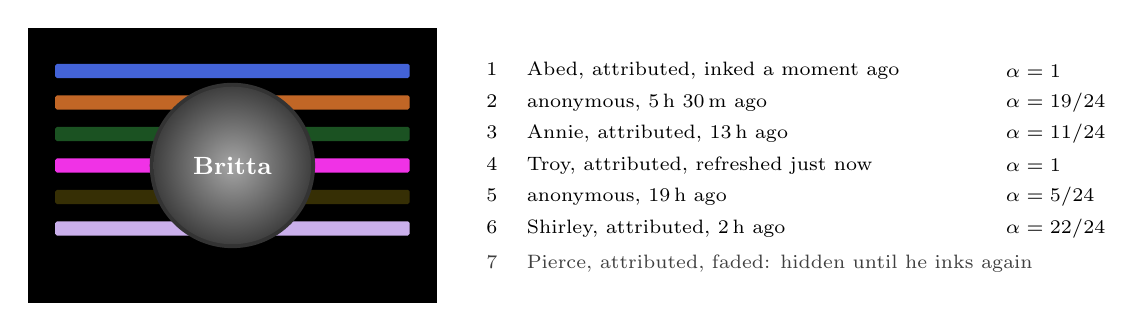
\begin{tikzpicture}[font=\scriptsize]
  \begin{scope}
    \fill[black] (-2.6,-1.75) rectangle (2.6,1.75);
    \stripe{1.20}{ink7}{1.00}{2.25}
    \stripe{0.80}{ink2}{0.79}{2.25}
    \stripe{0.40}{ink5}{0.46}{2.25}
    \stripe{0.00}{ink9}{1.00}{2.25}
    \stripe{-0.40}{ink3}{0.21}{2.25}
    \stripe{-0.80}{ink11}{0.92}{2.25}
    \fill[black!80] (0,0) circle (1.05);
    \shade[inner color=black!35,outer color=black!75] (0,0) circle (1.0);
    \node[text=white,font=\small\bfseries] at (0,0) {Britta};
  \end{scope}
  \begin{scope}[xshift=3.1cm,every node/.style={anchor=west,font=\scriptsize}]
    \foreach \y/\t/\a in {1.20/{1 \quad Abed, attributed, inked a moment ago}/{$\alpha=1$},
                          0.80/{2 \quad anonymous, 5\,h 30\,m ago}/{$\alpha=19/24$},
                          0.40/{3 \quad Annie, attributed, 13\,h ago}/{$\alpha=11/24$},
                          0.00/{4 \quad Troy, attributed, refreshed just now}/{$\alpha=1$},
                          -0.40/{5 \quad anonymous, 19\,h ago}/{$\alpha=5/24$},
                          -0.80/{6 \quad Shirley, attributed, 2\,h ago}/{$\alpha=22/24$}}
      { \node at (0,\y) {\t}; \node at (6.6,\y) {\a}; }
    \node[text=muted] at (0,-1.25) {7 \quad Pierce, attributed, faded: hidden until he inks again};
  \end{scope}
\end{tikzpicture}
\caption{Britta's flag, under the default decay of one step per hour over 24 hours. Stripe
locations are fixed by the order of first ink. A faded stripe takes no space, and comes back in
its place when refreshed.}
\label{fig:flag}
\end{figure}

\subsection{Who sees what}\label{sec:visibility}

The author of the game settled the rule: \emph{every player can see the full flag of every
other player who has declared their flag public.} A private flag is seen in full only by its
owner. Every inker can always see their own stripe on anyone.

\begin{center}\small
\begin{tabularx}{\linewidth}{@{}>{\raggedright\arraybackslash}p{38mm} X X@{}}
\toprule
viewer & a public flag & a private flag\\
\midrule
its owner & every stripe, its colour and history; names on attributed stripes & the same\\
another player & every stripe, its colour and history; names on attributed stripes & the viewer's own stripe only\\
a reader of the shard, without the game & every stripe and colour; inkers of attributed stripes & when each stripe changed; inkers of attributed stripes; no colours\\
\bottomrule
\end{tabularx}
\end{center}

Anonymous stripes carry no name for anyone. That includes the owner and readers of the shard,
subject to the relay's trust (\S\ref{sec:relay}).

\begin{decision}{D1}{What does private mean on the chain?}
\textbf{Settled by the author of the game:} each player declares their flag public or private,
and public flags are seen in full by everyone. \textbf{Recommended for the mechanism:} a
private flag's inks are sealed on the chain to two readers, the owner and the inker, with the
envelope F1R3Pix uses for messages (\S\ref{sec:sealing}). A public flag's inks are in the clear.
The environment refuses a clear ink on a private flag and a sealed ink on a public one, so the
form always matches the owner's choice at the block the ink lands in.

\textbf{Changing visibility.} Going public discloses the content key of each stripe's
\emph{current} sealed colour, and each stripe's earlier history stays sealed. Going private
seals inks from then on. It cannot unpublish colours already on the chain in the clear. The game
client stops showing them to other players, but a reader of the shard can still find them. The
client says so, in one line, when a player switches.

\textbf{Default.} Nothing is preselected. The entry dialogue asks the player to choose, and says
in one sentence what each choice shows to whom.
\end{decision}

\subsection{Attribution}

\begin{decision}{D2}{Who knows who inked whom?}
\textbf{Settled by the author of the game:} the inker declares whether their ink is attributed.
\textbf{Recommended for the details:}
\begin{itemize}[leftmargin=1.2em,itemsep=1pt]
\item Attribution belongs to the stripe, and is chosen at its first ink. A stripe cannot switch
  between attributed and anonymous ink by ink, because an attributed ink would expose every
  anonymous ink before and after it at the same location.
\item An attributed stripe is deployed by the inker. Its name is shown to everyone who can see
  the stripe.
\item An anonymous stripe is deployed by the F1R3Ink relay (\S\ref{sec:relay}), so the inker's
  address never appears on the chain against it.
\item An anonymous stripe may later be revealed by its inker. An attributed stripe cannot become
  anonymous, because its inker is already on the chain.
\item The client's default for a new stripe is \emph{attributed}, and the choice is one tap
  away beside the palette. A player can make anonymous their own default.
\item Anonymity among three people is not anonymity. The relay refuses anonymous inks in a round
  with fewer than \code{anonMin} entered participants (default 5), and the host may turn
  anonymous ink off.
\end{itemize}
\end{decision}

\subsection{Re-inking, lifting and history}

\begin{decision}{D3}{What happens when an inker inks the same person again?}
\textbf{Settled by the author of the game:} stripes are mutable, like the cells of F1R3Pix and
F1R3Beat. The inker's stripe keeps its location and takes the new colour. Every change is kept,
and right-clicking a stripe (or long-pressing it on a touch screen) shows its history of colours.
\textbf{Recommended additions:} re-inking with the same colour \emph{refreshes} the stripe, which
restarts its decay (D5). An inker may \emph{lift} their stripe, which removes its colour until
they ink again. The lift stays in the history. Each viewer sees a stripe's history at the same
visibility as the stripe itself.
\end{decision}

The history popover lists each change newest first: a swatch, the colour's palette number, how
long ago, and how faded it was when it was replaced. For an anonymous stripe, the popover shows
the history and no name.

\subsection{Colour}

\begin{decision}{D4}{Which colours may a stripe take?}
\textbf{Settled by the author of the game:} a palette. \textbf{Recommended:} the host chooses
the palette when creating the round, from 2 to 32 colours. The default is the sixteen below,
chosen to be far apart in hue and in lightness. On the chain an ink is a palette \emph{index},
which keeps sealed inks small and makes every colour comparable across a round.
\end{decision}

\begin{center}
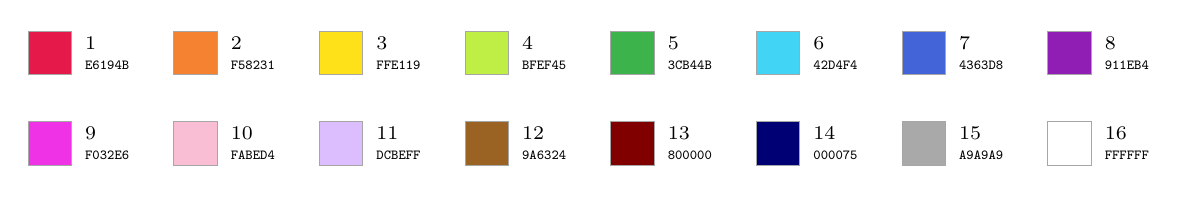
\begin{tikzpicture}[font=\scriptsize]
  \foreach \i in {1,...,16} {
    \pgfmathsetmacro{\x}{mod(\i-1,8)*1.85}
    \pgfmathsetmacro{\y}{-floor((\i-1)/8)*1.15}
    \fill[ink\i,draw=black!35,line width=0.3pt] (\x,\y) rectangle ++(0.55,0.55);
    \node[anchor=west] at (\x+0.6,\y+0.4) {\i};
  }
  \node[anchor=west,font=\tiny\ttfamily] at (0.6,0.12) {E6194B}; \node[anchor=west,font=\tiny\ttfamily] at (2.45,0.12) {F58231};
  \node[anchor=west,font=\tiny\ttfamily] at (4.3,0.12) {FFE119};  \node[anchor=west,font=\tiny\ttfamily] at (6.15,0.12) {BFEF45};
  \node[anchor=west,font=\tiny\ttfamily] at (8.0,0.12) {3CB44B};  \node[anchor=west,font=\tiny\ttfamily] at (9.85,0.12) {42D4F4};
  \node[anchor=west,font=\tiny\ttfamily] at (11.7,0.12) {4363D8}; \node[anchor=west,font=\tiny\ttfamily] at (13.55,0.12) {911EB4};
  \node[anchor=west,font=\tiny\ttfamily] at (0.6,-1.03) {F032E6}; \node[anchor=west,font=\tiny\ttfamily] at (2.45,-1.03) {FABED4};
  \node[anchor=west,font=\tiny\ttfamily] at (4.3,-1.03) {DCBEFF};  \node[anchor=west,font=\tiny\ttfamily] at (6.15,-1.03) {9A6324};
  \node[anchor=west,font=\tiny\ttfamily] at (8.0,-1.03) {800000};  \node[anchor=west,font=\tiny\ttfamily] at (9.85,-1.03) {000075};
  \node[anchor=west,font=\tiny\ttfamily] at (11.7,-1.03) {A9A9A9}; \node[anchor=west,font=\tiny\ttfamily] at (13.55,-1.03) {FFFFFF};
\end{tikzpicture}
\end{center}

Colours are identified by number and hex value, never by name. The March prototype named its
colours (rose, ember, ash, void), and a name such as ``ash'' suggests a meaning. In F1R3Ink the
meaning of a colour belongs to the community that uses it. Numbers also serve players who cannot
tell some colours apart: the swatch, its number and its hex value are always shown together.

\subsection{Decay}

\begin{decision}{D5}{How do stripes fade?}
\textbf{Settled by the author of the game:} colours grow more transparent with each configurable
unit of time, until they are refreshed or fade away completely. \textbf{Recommended for the
details:} the round fixes a unit $u$ and a number of steps $k$. A stripe last inked at block time
$t$ has, at time $\mathit{now}$, the opacity
\[
  \alpha \;=\; \max\!\Bigl(0,\; 1 - \frac{\lfloor(\mathit{now}-t)/u\rfloor}{k}\Bigr).
\]
It loses $1/k$ of its opacity at the end of each unit, and vanishes after $k$ units. Any ink by
the stripe's inker, including the same colour, resets $t$. A faded stripe keeps its location: it
takes no space on the flag, and it returns there when its inker inks again. The host may choose
no decay.
\end{decision}

\begin{figure}[h]
\centering
\begin{tikzpicture}[x=0.52cm,y=2.4cm,font=\scriptsize]
  \draw[->,black!60] (0,0) -- (25.5,0) node[right]{hours since last ink};
  \draw[->,black!60] (0,0) -- (0,1.15) node[above]{$\alpha$};
  \foreach \h in {0,4,...,24} \draw[black!40] (\h,0) -- (\h,-0.03) node[below]{\h};
  \foreach \a in {0.25,0.5,0.75,1} \draw[black!40] (0,\a) -- (-0.25,\a) node[left]{\a};
  \foreach \s in {0,...,23} {
    \pgfmathsetmacro{\a}{1-\s/24}
    \draw[brandskydark,line width=0.9pt] (\s,\a) -- (\s+1,\a);
  }
  \draw[brandskydark,line width=0.9pt] (24,0) -- (25.3,0);
  \fill[brandyellow] (5.5,{19/24}) circle (2.2pt);
  \draw[black!50,line width=0.4pt] (5.6,{19/24+0.02}) -- (8.45,1.0);
  \node[anchor=west] at (8.5,1.0) {stripe 2 of Figure~\ref{fig:flag}: $\lfloor 5.5\rfloor=5$, so $\alpha=19/24$};
\end{tikzpicture}
\caption{Opacity under the default decay, \emph{a day}: one step per hour, over 24 steps.}
\label{fig:decay}
\end{figure}

\begin{center}\small
\begin{tabular}{@{}lllll@{}}
\toprule
preset & unit $u$ & steps $k$ & gone after & suits\\
\midrule
an evening & 10 minutes & 12 & 2 hours & a game played in one sitting\\
a day (default) & 1 hour & 24 & 24 hours & a team or a class over a day\\
a week & 6 hours & 28 & 7 days & a community over a week\\
a season & 1 day & 90 & 90 days & a long-lived community\\
never & --- & --- & --- & a round where every ink stands\\
\bottomrule
\end{tabular}
\end{center}

Decay is not computed on the chain. The chain records when each stripe was last inked, by the
block's timestamp, and every reader derives $\alpha$ from it. All readers at the same block
therefore agree. Between blocks, the client advances $\mathit{now}$ by its own clock, but never
past the next block it sees. When a round closes, $\mathit{now}$ stops at the closing block. A
closed round's flags stay as they were at the close.

\subsection{Phases}

F1R3Ink uses the Portal's instance status (\code{lobby}, \code{active}, \code{closed}), set
only by the host.

\begin{decision}{D6}{What may players do in each phase?}
\textbf{Recommendation.}

\begin{tabular}{@{}lcccccc@{}}
\toprule
 & enter & tags, visibility & ink & message & pay & read\\
\midrule
\code{lobby}  & yes & yes & no  & yes & yes & yes\\
\code{active} & yes & yes & yes & yes & yes & yes\\
\code{closed} & no  & no  & no  & no  & no  & yes\\
\bottomrule
\end{tabular}\par\medskip

The lobby lets players gather, describe themselves, choose their visibility and talk before
anyone is inked, so that a round starts together. Closing freezes every flag, its decay included.
\end{decision}

\begin{decision}{D7}{How large is a round?}
\textbf{Recommendation:} the host sets a capacity when creating the round, from 3 to 64
participants, with a default of 24. A flag has at most one stripe per other participant, so
capacity bounds both a flag's height and the cost of reading every flag
(\S\ref{sec:reads}). The upper bound is provisional, and Phase~4 measures it
(\S\ref{sec:plan}). A participant who leaves through the Portal keeps the stripes they gave,
which go on fading. Their own flag stays as it was, and no one can ink them until they rejoin.
\end{decision}

% ================================================================= 4
\section{Rewarding disclosure}\label{sec:incentives}

The game works only if enough flags are public. A private flag still tells its owner how the
community sees them, but it teaches the community nothing about itself. The author of the game
asked what, beyond a more fulfilling game, might encourage disclosure. The proposals below avoid
the incentive that would damage the game, which is paying for colours. A reward for disclosure
should reward \emph{showing} a flag, never what is on it, so that no one has a reason to ink for
effect.

\begin{decision}{D8}{What rewards a public flag?}
\textbf{Recommendation: the first three in version 1, the fourth as a host option, the fifth
later.}
\begin{enumerate}[leftmargin=1.4em,itemsep=2pt]
\item \textbf{The commons.} The community spectrum (\S\ref{sec:aggregates}) is built from
  public flags only, and it says so in its header: ``14 of 22 flags''. Going public visibly adds
  a person to the picture the community has of itself. Going private visibly takes them out.
\item \textbf{The portrait.} Only a flag's owner may publish it to the gallery as a \code{flag}
  play (\S\ref{sec:gallery}). The portrait is a record of how a community saw someone, which
  others can view and react to. A private flag can be published too, which discloses it, and
  the act of publishing is the owner's to choose.
\item \textbf{The conversation.} The owner of a public flag can see who holds each attributed
  stripe, and so can everyone else. That makes the flag an opening for conversation, by message,
  about why someone chose a colour. Many players will find that the richest part of the game.
\item \textbf{Show to see} (host option, \code{reciprocity}, off by default). Under this
  option, only a player whose own flag is public sees other public flags in full. A player whose
  flag is private sees only their own stripes and the counts. This is the strongest incentive
  here, but it narrows the settled rule that every player sees every public flag. It is
  therefore offered to hosts and not imposed. It is also enforced only by the client: public
  colours are on the chain in the clear, and a reader of the shard can see them regardless.
\item \textbf{A stipend for disclosure} (later). A sponsor could fund a stipend paid at the close
  to every player whose flag was public for the whole round, through the Portal's
  \code{sponsors} domain. The stipend pays for showing a flag, not for its colours. It needs the
  Portal's sponsorship terms to ask the game environment about disclosure, which they cannot do
  today, so it is left for a later version.
\end{enumerate}
\end{decision}

% ================================================================= 5
\section{Architecture}\label{sec:arch}

F1R3Ink adds one new kind of component to what F1R3Pix and F1R3Beat use: a \emph{relay}, which
deploys anonymous inks for their inkers. Everything else is one game environment on the shard,
one game client framed by the Portal shell, and the Portal's existing \code{payments} domain and
host protocol, which gains a \code{relay} method.

\begin{figure}[ht]
\centering
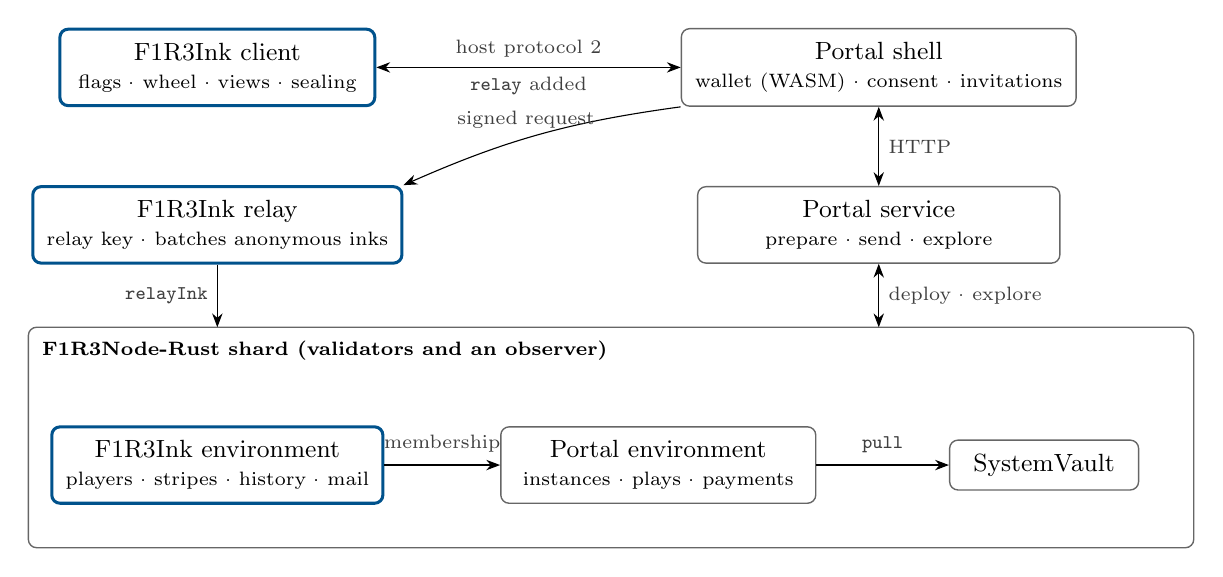
\begin{tikzpicture}[font=\small,
  box/.style={draw=black!60,line width=0.5pt,rounded corners=3pt,align=center,inner sep=5pt,fill=white},
  new/.style={box,draw=brandskydark,line width=1.1pt},
  lab/.style={font=\scriptsize,text=muted,align=center},
  >={Stealth[length=5pt]}]
  \node[new,minimum width=40mm] (game) at (0,0) {F1R3Ink client\\[-1pt]{\scriptsize flags · wheel · views · sealing}};
  \node[box,minimum width=46mm] (shell) at (8.4,0) {Portal shell\\[-1pt]{\scriptsize wallet (WASM) · consent · invitations}};
  \node[box,minimum width=46mm] (svc) at (8.4,-2.0) {Portal service\\[-1pt]{\scriptsize prepare · send · explore}};
  \node[new,minimum width=40mm] (relay) at (0,-2.0) {F1R3Ink relay\\[-1pt]{\scriptsize relay key · batches anonymous inks}};
  \draw[black!60,rounded corners=3pt,line width=0.5pt] (-2.4,-3.3) rectangle (12.4,-6.1);
  \node[anchor=north west,font=\scriptsize\bfseries] at (-2.35,-3.35) {F1R3Node-Rust shard (validators and an observer)};
  \node[new,minimum width=36mm] (ienv) at (0,-5.05) {F1R3Ink environment\\[-1pt]{\scriptsize players · stripes · history · mail}};
  \node[box,minimum width=40mm] (penv) at (5.6,-5.05) {Portal environment\\[-1pt]{\scriptsize instances · plays · payments}};
  \node[box,minimum width=24mm] (vault) at (10.5,-5.05) {SystemVault};
  \draw[<->] (game) -- node[above,lab]{host protocol 2} node[below,lab]{\code{relay} added} (shell);
  \draw[<->] (shell) -- node[right,lab]{HTTP} (svc);
  \draw[<->] (svc) -- node[right,lab]{deploy · explore} (8.4,-3.3);
  \draw[->] (shell.south west) to[bend right=8] node[above,lab,pos=0.55]{signed request} (relay.north east);
  \draw[->] (relay) -- node[left,lab]{\code{relayInk}} (0,-3.3);
  \draw[->] (ienv) -- node[above,lab,yshift=1pt]{membership} (penv);
  \draw[->] (penv) -- node[above,lab,yshift=1pt]{\code{pull}} (vault);
\end{tikzpicture}
\caption{Components. Outlined in dark sky: what this design adds or replaces.}
\label{fig:arch}
\end{figure}

\subsection{Authority}

\begin{itemize}[leftmargin=1.2em,itemsep=2pt]
\item The game client never sees a key. It reaches identity, the shard, payment and the relay
  only through the host protocol.
\item The F1R3Ink environment reads two things and nothing else. The first is the caller's
  address, which it obtains from \code{rho:deploy:data} through \code{rho:vault:\allowbreak address}, and the second is the block's
  number and timestamp, from \code{rho:block:data}. It never touches a vault.
\item Funds move only through the Portal environment's \code{payments.send}, signed only from
  the Portal shell after a prompt.
\item Sealed colours are sealed in the game client and opened by the wallet. The chain holds only
  ciphertext.
\item The relay holds one key, the \emph{relay key}, which the F1R3FLY.io Cooperative names in
  the F1R3Ink environment, as it names F1R3Beat's breeder. That key can write and reveal
  anonymous stripes, and nothing else. Unlike the breeder, the relay is trusted: it knows who
  holds each anonymous stripe (\S\ref{sec:relay}).
\end{itemize}

% ================================================================= 6
\section{The F1R3Ink environment}\label{sec:env}

The environment replaces the installed \code{f1r3ink.rho} body inside the shared game
\code{prelude.rho}. It keeps the prelude's machinery: installation under the game's registry
key with \code{rho:registry:\allowbreak insertSigned:\allowbreak secp256k1}, version-checked upgrade, \code{who},
\code{member}, \code{instanceOf} and the \code{TreeHashMap} store. Installing it raises the
environment's version. The URI is unchanged, every call template's hash changes, and the F1R3FLY.io
Cooperative re-registers the manifest (\S\ref{sec:manifest}).

\subsection{Configuration}

The configuration is the \code{config} map the host passes to the Portal's
\code{instances.create}. It is read from the Portal's instance record and fixed at creation.

\begin{lstlisting}[language=rholang]
{ "capacity":     24,                 // 3 ..= 64                                     (D7)
  "palette":      ["#E6194B", ...],   // 2 ..= 32 distinct "#RRGGBB", upper case      (D4)
  "decay":        { "unit": 3600000, "steps": 24 },   // ms and count, or Nil         (D5)
  "minInterval":  60000,              // ms between inks on one stripe               (D9)
  "anonymous":    true,               // may stripes be anonymous?                    (D2)
  "anonMin":      5,                  // entered participants needed for anonymity    (D2)
  "reciprocity":  false,              // "show to see"                               (D8)
  "messageLimit": 2048 }              // bytes of sealed envelope per message     (sec. 9)
\end{lstlisting}

\req{r:config}~The environment \MUST{} refuse every move on an instance whose configuration is
missing or out of range, answering \code{(false, "bad config")}. It \MUSTNOT{} substitute
defaults. Defaults are applied by the client that creates the instance, where the host can see
them.

\subsection{State}

Every key is scoped by instance, and every key has exactly one writer.

\begin{center}\small
\begin{tabularx}{\linewidth}{@{}>{\ttfamily}l X l@{}}
\toprule
\normalfont key & value & writer\\
\midrule
("p", i, a)        & \code{\{"pk", "flag": "public"|"private", "tags": [...], "veil": [sid, ...], "at": [h, t]\}} & $a$\\
("plog", i, a)     & list of \code{[h, t, "flag", v]} and \code{[h, t, "tags", tags]}, oldest first & $a$\\
("disc", i, a)     & list of \code{[sid, seq, K]}: content keys $a$ disclosed on going public & $a$\\
("s", i, b, sid)   & stripe: \code{\{"by": a | Nil, "first": [h, t], "last": [h, t], "seq": n, "ink"\}} & inker, or relay\\
("sh", i, b, sid)  & the stripe's history: list of \code{[h, t, ink]} & inker, or relay\\
("o", i, a)        & the set of targets $a$ has inked & $a$\\
("o", i, "relay")  & map from target to the set of anonymous handles on them & relay\\
("out", i, a)      & sealed messages sent by $a$, as F1R3Pix & $a$\\
\bottomrule
\end{tabularx}
\end{center}

Here $b$ is the target, $h$ a block number and $t$ a block timestamp. A stripe id \code{sid} is
the inker's address for an attributed stripe, or \code{["anon", handle]} for an anonymous one. An
\code{ink} is \code{\{"c": n\}} (palette index $n$, in the clear), \code{\{"sealed": bytes\}}
(an envelope, \S\ref{sec:sealing}), or \code{Nil} (lifted).

\req{r:single-writer}~Every key \MUST{} have the single writer shown. An inker writes only their
own stripes and their own index, and the relay writes only anonymous stripes and its own index.
Two players inking the same target therefore never contend for a key, which fixes Finding~3. The
environment keeps no instance-wide counter or log. Global order is recovered when reading
(\S\ref{sec:order}).

\subsection{Moves}\label{sec:moves}

Moves are play templates. Within the allowance granted at launch they are signed without a
prompt. Each answers \code{(true, value)} or \code{(false, reason)}.

\textbf{\code{enter(instance, pk, flag)}.} Registers the caller. \code{pk} is their
uncompressed secp256k1 public key, used to seal inks and messages to them, and \code{flag} is
\code{"public"} or \code{"private"}.
\begin{itemize}[leftmargin=1.2em,itemsep=1pt]
\item Refuses unless the caller is a participant and the status is not \code{closed}.
\item Refuses unless \code{rho:vault:address}'s \code{"fromPublicKey"} applied to \code{pk}
  yields the caller's address.
\item If the caller has already entered, answers their record unchanged.
\item Refuses with \code{"full"} if the round already has \code{capacity} entered participants.
\end{itemize}

\textbf{\code{tags(instance, tags)}.} Replaces the caller's tags and appends the change to their
log. Refuses unless the caller has entered and the status is not \code{closed}. A list may hold
at most 12 tags, each 1 to 24 characters with no control characters.

\textbf{\code{visibility(instance, flag, keys)}.} Sets the caller's flag to \code{"public"} or
\code{"private"} and appends the change to their log. Going public requires \code{keys}, the
content key of the current envelope of every sealed stripe on the caller's flag. The
environment appends them to \code{("disc", i, a)}. It cannot check them, because it cannot run
AES-GCM. Every client checks a disclosed key against its envelope, and a stripe whose key is
missing or wrong is drawn veiled, with a mark saying the owner did not disclose it. Going private
takes \code{Nil}.

\textbf{\code{ink(instance, target, ink)}.} Sets the caller's attributed stripe on
\code{target}.
\begin{itemize}[leftmargin=1.2em,itemsep=1pt]
\item Refuses unless the caller and the target are both entered participants, the target is not
  the caller, and the status is \code{active}.
\item Refuses unless \code{ink} has the form the target's flag requires: \code{\{"c": n\}} with
  $0\le n<|\mathit{palette}|$ for a public flag, or \code{\{"sealed": bytes\}} of at most 320
  bytes for a private flag. \code{Nil} (a lift) is accepted for either.
\item Reads the block's number $h$ and timestamp $t$. If the stripe exists, refuses with
  \code{"too soon"} unless $t \ge t_{\mathit{last}} + \mathit{minInterval}$.
\item Writes the stripe (creating it with \code{first} $=[h, t]$ if it is new), sets
  \code{last} $=[h,t]$, increments \code{seq}, appends \code{[h, t, ink]} to its history, and adds
  the target to the caller's index. Answers \code{\{"sid", "seq", "h", "t"\}}.
\end{itemize}

\textbf{\code{veil(instance, sids)}.} Sets the list of stripes on the caller's own public flag
that the client hides from other players (D15). The stripes' colours stay on the chain.

\textbf{\code{say(instance, to, envelope)}.} As F1R3Pix's \code{say}, with recipients drawn
from the entered participants.

\textbf{Relay moves.} Two moves are signed only by the relay key, from the relay, and are not
game templates.
\begin{itemize}[leftmargin=1.2em,itemsep=1pt]
\item \code{relayInk(instance, batch)}, where \code{batch} is a list of up to 64
  \code{[target, handle, ink]}. Each entry is checked as \code{ink} checks it, against the
  stripe \code{["anon", handle]}, and also against \code{anonymous} and \code{anonMin}. Entries
  are independent: the move answers one result per entry.
\item \code{relayReveal(instance, target, handle, address)} sets the \code{by} of an anonymous
  stripe, revealing its inker. The stripe keeps its id, location and history.
\end{itemize}
\code{setRelay(address)}, signed only by the holder of the F1R3Ink registry key, names the
relay, as F1R3Beat's \code{setBreeder} names the breeder.

\subsection{Reads}\label{sec:reads}

Reads are explore deploys served by the observer. They cost the reader nothing and need no
signature.

\begin{center}\small
\begin{tabularx}{\linewidth}{@{}>{\ttfamily}l X@{}}
\toprule
\normalfont template & answers\\
\midrule
f1r3ink.players(instance)   & every entered participant: \code{pk}, \code{flag}, \code{tags}, \code{veil}, \code{at}\\
f1r3ink.flags(instance)     & every stripe, grouped by target: \code{sid}, \code{by}, \code{first}, \code{last}, \code{seq} and the current \code{ink}; with every \code{("disc", ...)} list\\
f1r3ink.history(instance, target, sid, from) & a stripe's history from position \code{from}, up to 256 entries\\
f1r3ink.log(instance, from, to) & every ink, tag change and visibility change with $\mathit{from}\le h<\mathit{to}$, in the order of \S\ref{sec:order}\\
f1r3ink.mail(instance, address, cursor), outbox(\ldots) & as F1R3Pix\\
\bottomrule
\end{tabularx}
\end{center}

\code{flags} reads each participant's index and then only the stripes that exist, so it touches
$n + S$ keys for $n$ participants and $S$ stripes. At the default capacity that is at most
$24 + 24\cdot 23 = 576$, and at 64 it is at most 4{,}096. Phase~4 measures whether the upper
bound holds as a single read.

\req{r:now}~Every read result \MUST{} carry the number, hash and timestamp of the block it
reflects. The Portal service adds the timestamp, which it reads from the block's header. The
client takes $\mathit{now}$ for decay from it (D5).

\subsection{Order and time}\label{sec:order}

An ink is stamped with the number and timestamp of the block that includes it, from
\code{rho:block:data}. Decay runs on the block's timestamp and not on the deploy's, because the
deploy timestamp is chosen by the inker, who could otherwise keep a stripe artificially fresh.
The block timestamp is chosen by the proposing validator. History is ordered by block number,
then by deploy timestamp within the block, then by target, then by stripe id.

\subsection{A sketch of \code{ink}}

\begin{lstlisting}[language=rholang]
contract env(@"ink", @instance, @target, @ink, ret) = {
  new whoCh, rCh, cCh, gCh, sCh, ack1, ack2, ack3 in {
    who!(*whoCh) |
    for (@by, _ <- whoCh) {
      // config valid? both entered participants? not self? "active"?
      // form of ink matches the target's flag, and index in the palette?
      inkReady!(instance, by, target, ink, *rCh) |
      for (@ok, @why <- rCh) {
        if (not ok) { ret!((false, why)) }
        else {
          clock!(*cCh) |                          // rho:block:data
          gapOf!(instance, *gCh) |                // minInterval
          TreeHashMap!("get", state, key, *sCh) | // key = ("s", instance, target, by)
          for (@h, @t <- cCh & @gap <- gCh & @stripe <- sCh) {
            match stripe {
              Nil => {
                put!(key, {"by": by, "first": [h, t], "last": [h, t],
                           "seq": 1, "ink": ink}, *ack1)
              }
              _ => {
                if (t < stripe.get("last").nth(1) + gap) {
                  ret!((false, "too soon"))
                } else {
                  put!(key, stripe.set("last", [h, t])
                                  .set("seq", stripe.get("seq") + 1)
                                  .set("ink", ink), *ack1)
                }
              }
            } |
            for (_ <- ack1) {
              append!(("sh", instance, target, by), [h, t, ink], *ack2) |
              addTarget!(("o", instance, by), target, *ack3) |
              for (_ <- ack2 & _ <- ack3) {
                ret!((true, {"sid": by, "h": h, "t": t}))
              }
            }
          }
        }
      }
    }
  }
}
\end{lstlisting}

\code{inkReady}, \code{clock}, \code{put}, \code{append} and \code{addTarget} are prelude-level
helpers. \code{gapOf} reads \code{minInterval} from the configuration, and \code{key} stands
for \code{("s", instance, target, by)}.
\code{relayInk} runs the same body for each entry, with \code{["anon", handle]} as the stripe id
and \code{"by": Nil}.

\subsection{Pacing}

\begin{decision}{D9}{How often may one person ink another?}
\textbf{Recommendation:} at most once per \code{minInterval} per stripe (default one minute of
block time), enforced on the chain. The client also coalesces inks, as F1R3Pix coalesces paints:
while one ink is in flight, further choices replace a single queued ink. Browsing the palette
therefore costs one deploy. The interval stops one player from flickering a stripe to draw
attention, and it bounds the history at roughly one entry per minute per stripe.
\end{decision}

% ================================================================= 7
\section{Sealing private flags}\label{sec:sealing}

A private flag's inks use the envelope F1R3Pix defined for messages, with two changes.

\begin{enumerate}[leftmargin=1.4em,itemsep=2pt]
\item \textbf{Domain.} The \code{info} and \code{aad} strings are \code{"f1r3ink/ink/v1"}, and the
  \code{aad} binds the instance, the target, the stripe id and the stripe's next \code{seq}. A
  sealed ink cannot be replayed onto another stripe or into another position of its own history.
\item \textbf{Unlabelled wraps.} A message envelope labels each wrap of the content key with its
  recipient's address. A sealed ink has exactly two wraps, one for the target and one for the
  inker, and both are unlabelled and in random order. Each reader tries both. An anonymous stripe
  would otherwise name its inker in its own envelope. All sealed inks use unlabelled wraps, so
  that attributed and anonymous inks look alike.
\end{enumerate}

The plaintext is the palette index as one byte, padded to a fixed 16 bytes, so every sealed ink
has the same length. The envelope comes to about 250 bytes, within the 320-byte bound of
\code{ink}. Phase~1 fixes the exact layout against test vectors.

\req{r:open-unlabelled}~The host's \code{open} \MUST{} accept envelopes with unlabelled wraps,
trying each wrap with the active key, and \MUST{} bind the hosted game and instance as F1R3Pix's
R4 requires. It answers \code{not-addressed} when no wrap opens.

\textbf{Disclosure.} Going public discloses the content key $K$ of each stripe's current sealed
ink, which the owner obtains by opening it. Anyone holding $K$ can decrypt that one envelope and
check it against the chain, and nothing else. The stripe's earlier inks stay sealed. A disclosed
colour is as verifiable as a clear one.

% ================================================================= 8
\section{The relay}\label{sec:relay}

Finding~8 leaves one way to make an ink anonymous on a public chain: someone other than the inker
deploys it. The relay is that someone. It is a small service, run by the F1R3FLY.io Cooperative
beside the Portal service, that holds the relay key and pays the phlo for anonymous inks.

\begin{figure}[h]
\centering
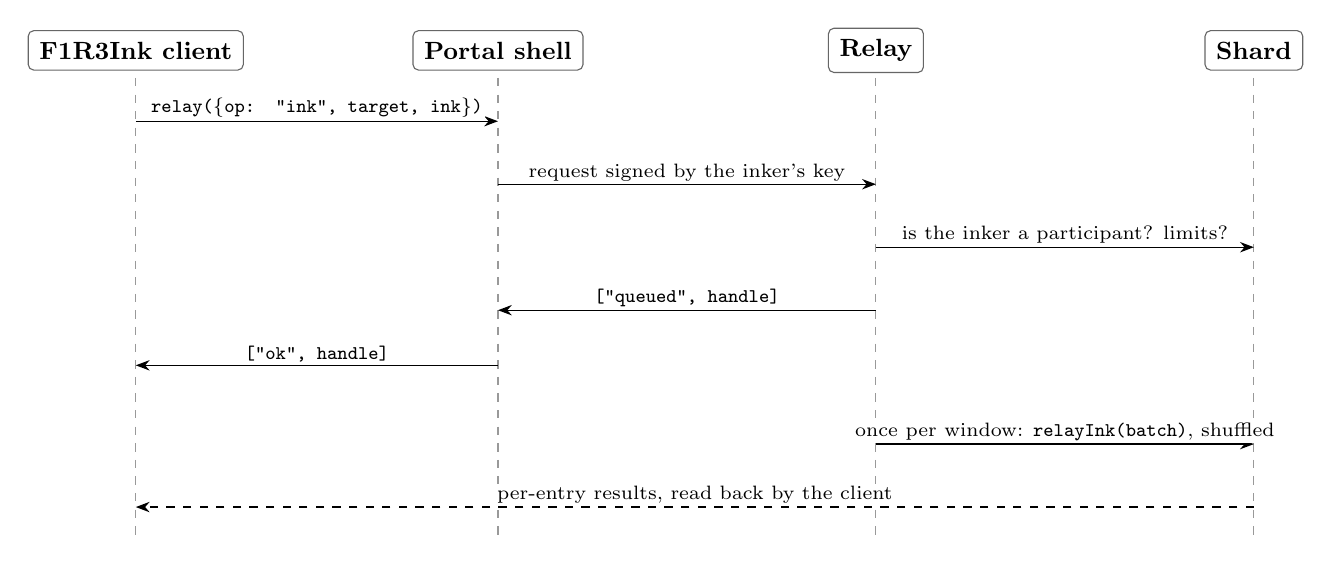
\begin{tikzpicture}[font=\small,>={Stealth[length=5pt]},
  life/.style={draw=black!40,dashed},
  hd/.style={draw=black!60,rounded corners=2pt,fill=white,inner sep=4pt,font=\small\bfseries},
  msg/.style={->,line width=0.5pt},
  lab/.style={font=\scriptsize,fill=white,inner sep=1pt}]
  \foreach \x/\n/\t in {0/g/F1R3Ink client,4.6/s/Portal shell,9.4/r/Relay,14.2/c/Shard}{
    \node[hd] (\n) at (\x,0) {\t};
    \draw[life] (\x,-0.35) -- (\x,-6.2);
  }
  \draw[msg] (0,-0.9) -- node[lab,above]{\code{relay(\{op: "ink", target, ink\})}} (4.6,-0.9);
  \draw[msg] (4.6,-1.7) -- node[lab,above]{request signed by the inker's key} (9.4,-1.7);
  \draw[msg] (9.4,-2.5) -- node[lab,above]{is the inker a participant? limits?} (14.2,-2.5);
  \draw[msg] (9.4,-3.3) -- node[lab,above]{\code{["queued", handle]}} (4.6,-3.3);
  \draw[msg] (4.6,-4.0) -- node[lab,above]{\code{["ok", handle]}} (0,-4.0);
  \draw[msg] (9.4,-5.0) -- node[lab,above]{once per window: \code{relayInk(batch)}, shuffled} (14.2,-5.0);
  \draw[msg,dashed] (14.2,-5.8) -- node[lab,above]{per-entry results, read back by the client} (0,-5.8);
\end{tikzpicture}
\caption{An anonymous ink. The inker's address goes to the relay and never to the chain.}
\label{fig:relayflow}
\end{figure}

\textbf{Requests.} The game asks the shell to relay a request. The shell signs it with the
inker's identity key under the domain \code{"f1r3games/relay/v1"} together with the game id, the
instance and the relay's URL from the manifest, and posts it to the relay. The relay checks the
signature and the inker's participation, and queues the ink.

\textbf{Handles.} The relay derives each stripe's handle as
\[
  \mathit{handle} = \mathrm{HMAC\text{-}SHA256}\bigl(s_{\mathit{relay}},\ \text{\code{"f1r3ink/handle/v1"}} \,\|\, \mathit{instance} \,\|\, \mathit{target} \,\|\, \mathit{inker}\bigr)_{0..16},
\]
with a secret $s_{\mathit{relay}}$ that it keeps. The same inker on the same target always gets
the same stripe, and the relay keeps no table. The inker's client learns its handle from the
relay's answer, and can ask for it again with a signed request.

\textbf{Batching.} The relay submits at most one \code{relayInk} per window, three blocks by
default, carrying every ink queued in that window in random order. That blurs when an anonymous
ink was given to within a window. It cannot hide it from a target who knows that only one person
was online.

\textbf{Limits.} The relay applies \code{minInterval} before queueing, so a refused ink is
refused at once. It caps each inker at 30 relayed inks per hour, so that the Cooperative's phlo
cannot be drained through it. If an entry is refused because its target changed visibility
after the request, the relay returns it to the inker's client, which seals or unseals the ink
and asks again.

\begin{decision}{D10}{How much must players trust the relay?}
\textbf{Recommendation: accept a trusted relay in version 1, and say so.} The relay sees who
inks whom, and for public flags, with which colour. It cannot read a sealed colour, and it
cannot forge an ink, because every request carries the inker's signature, which the relay keeps
and which an auditor can demand. The trust it needs is the trust the Cooperative already holds
as the registry's governor. Removing that trust needs anonymous credentials, with which a
participant proves membership of the round without saying which member they are. That means ring
signatures, blind signatures or a zero-knowledge membership proof, and F1R3Node-Rust offers none
of them as a system process today. The client explains this in the anonymity toggle's help: an
anonymous ink is hidden from every player and every reader of the shard, but not from the
F1R3FLY.io Cooperative.
\end{decision}

\req{r:relay-cap}~\code{relay} \MUST{} be a declared capability, and the shell \MUST{} post only
to the relay URL in the hosted game's registered manifest. A game frame cannot use it to obtain
the inker's signature for any other purpose.

% ================================================================= 9
\section{Messages and payments}\label{sec:mail}

\begin{decision}{D11}{How do players talk and pay?}
\textbf{Settled by the author of the game: include both. Recommended: exactly as F1R3Pix (its
D6, D7 and D10) and F1R3Beat (its D8).} Messages are on the chain and sealed to their recipients
and the sender, with the domain string \code{"f1r3ink/msg/v1"}. Payments go through the Portal
environment's \code{payments.send}, signed only from the shell after a prompt, with \emph{each}
as the default and \emph{split} on request. The manifest declares
\code{"capabilities": ["pay", "open", "relay"]}.
\end{decision}

The same requirements apply: the host binds the game id and instance into \code{open}, refuses a
\code{pay} that names a non-participant before prompting, and never signs \code{payments.send}
within an allowance. Messages to an anonymous inker are out of scope for version 1
(\S\ref{sec:future}). A player can message only the people they can name.

% ================================================================= 10
\section{Host protocol additions}\label{sec:host}

\begin{center}\small
\begin{tabularx}{\linewidth}{@{}>{\ttfamily}l X@{}}
\toprule
\normalfont method & behaviour\\
\midrule
relay(\{op, ...\}) & New, declared. Signs the request with the active key under the domain of R\ref{r:relay-cap}, posts it to the manifest's \code{relay} URL, and answers the relay's reply. Counts against the launch allowance like a play move, and never prompts within it. Errors: \code{no-relay}, \code{relay}, \code{allowance}.\\
open(\{envelope\}) & Extended to unlabelled wraps (R\ref{r:open-unlabelled}). Unchanged otherwise.\\
\bottomrule
\end{tabularx}
\end{center}

The relay's operations are \code{ink} (target, ink), \code{reveal} (target) and \code{handles}
(instance), which lists the caller's own handles. The Portal environment gains one record: when
\code{instances.setStatus} changes an instance's status, it records the block number and
timestamp under \code{statusAt}, so that every reader agrees on when the round closed (D5).
Neither addition is specific to F1R3Ink.

% ================================================================= 11
\section{The client}\label{sec:client}

The client is a web page served from the game's own origin and framed by the Portal. Like the
F1R3Pix and F1R3Beat clients, it has a framework-free TypeScript core holding every operation
and a React layer that only renders, so that each core operation can later become a f1r3lang
process in F1R3Gaze.

\subsection{Layout}

The page keeps the deck's two columns. Messaging and tokens are added to the left column,
beneath the player's own flag, and do not get a third column.

\begin{figure}[h]
\centering
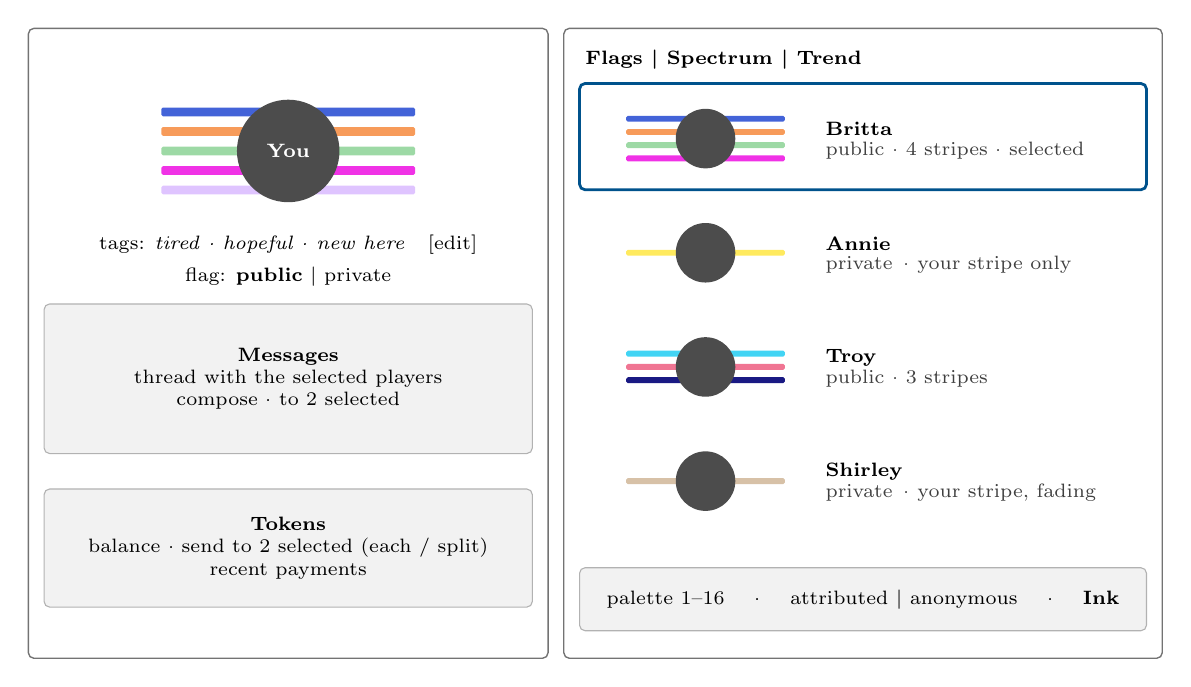
\begin{tikzpicture}[font=\scriptsize,
  col/.style={draw=black!55,line width=0.5pt,rounded corners=2pt},
  pane/.style={draw=black!30,rounded corners=2pt,fill=codebg,align=center,inner sep=2pt}]
  \draw[col] (0,0) rectangle (6.6,8.0);
  \draw[col] (6.8,0) rectangle (14.4,8.0);
  % left
  \begin{scope}[shift={(3.3,6.35)},scale=0.62]
    \stripe{0.95}{ink7}{1}{2.6}\stripe{0.55}{ink2}{0.8}{2.6}\stripe{0.15}{ink5}{0.5}{2.6}
    \stripe{-0.25}{ink9}{1}{2.6}\stripe{-0.65}{ink11}{0.9}{2.6}
    \fill[black!70] (0,0.15) circle (1.05);
    \node[text=white,font=\scriptsize\bfseries] at (0,0.15) {You};
  \end{scope}
  \node[font=\scriptsize] at (3.3,5.25) {tags: \emph{tired · hopeful · new here}\quad[edit]};
  \node[font=\scriptsize] at (3.3,4.85) {flag: \textbf{public} \textbar{} private};
  \node[pane,minimum width=62mm,minimum height=19mm] at (3.3,3.55) {\textbf{Messages}\\thread with the selected players\\compose · to 2 selected};
  \node[pane,minimum width=62mm,minimum height=15mm] at (3.3,1.4) {\textbf{Tokens}\\balance · send to 2 selected (each / split)\\recent payments};
  % right
  \node[anchor=north west,font=\scriptsize\bfseries] at (6.95,7.85) {Flags \textbar{} Spectrum \textbar{} Trend};
  \foreach \y/\n/\s in {6.6/Britta/1,5.15/Annie/2,3.7/Troy/3,2.25/Shirley/4} {
    \begin{scope}[shift={(8.6,\y)},scale=0.42]
      \ifnum\s=1 \stripe{0.6}{ink7}{1}{2.4}\stripe{0.2}{ink2}{0.8}{2.4}\stripe{-0.2}{ink5}{0.5}{2.4}\stripe{-0.6}{ink9}{1}{2.4}\fi
      \ifnum\s=2 \stripe{0.0}{ink3}{0.7}{2.4}\fi
      \ifnum\s=3 \stripe{0.4}{ink6}{1}{2.4}\stripe{0.0}{ink1}{0.6}{2.4}\stripe{-0.4}{ink14}{0.9}{2.4}\fi
      \ifnum\s=4 \stripe{0.0}{ink12}{0.4}{2.4}\fi
      \fill[black!70] (0,0) circle (0.9);
    \end{scope}
    \node[anchor=west] at (10.0,\y+0.12) {\textbf{\n}};
  }
  \node[anchor=west,text=muted] at (10.0,6.45) {public · 4 stripes · selected};
  \node[anchor=west,text=muted] at (10.0,5.0) {private \,· your stripe only};
  \node[anchor=west,text=muted] at (10.0,3.55) {public · 3 stripes};
  \node[anchor=west,text=muted] at (10.0,2.1) {private \,· your stripe, fading};
  \draw[brandskydark,line width=1pt,rounded corners=2pt] (7.0,5.95) rectangle (14.2,7.3);
  \node[pane,minimum width=72mm,minimum height=8mm] at (10.6,0.75) {palette 1--16 \quad · \quad attributed \textbar{} anonymous \quad · \quad \textbf{Ink}};
\end{tikzpicture}
\caption{The two columns. Left: you, your flag, your tags and your visibility, then messages and
tokens. Right: the wheel, which can switch to the aggregate views, with the ink control for the
selected player.}
\label{fig:layout}
\end{figure}

\textbf{Left column: you.} Your avatar with your full flag behind it, your tags (edited in
place), and your flag's visibility, with a one-line reminder of who can see it. Beneath them are
the message thread with the selected players and the token controls, which work exactly as in
F1R3Pix: the send control targets the selected players and shows \emph{each} or \emph{split}
with the total.

\textbf{Right column: everyone else.} A vertical wheel of the other entered players' avatars,
drawn from Portal profiles. The avatar at the wheel's focus is full size, and avatars shrink
with distance from it. Each avatar carries the stripes the viewer may see (\S\ref{sec:visibility}):
a public flag in full, a private flag as the viewer's own stripe alone, with a small lock. The
viewer's own stripe on a public flag is marked with a notch at its left end. Selecting players
drives the message and payment recipients. Selecting exactly one player opens the ink control
beneath the wheel: the palette, the attribution toggle for a new stripe, and \textbf{Ink}. The
wheel's header switches the column between \emph{Flags} (the wheel), \emph{Spectrum} and
\emph{Trend} (\S\ref{sec:aggregates}), and holds \emph{Invite}, which opens the Portal's shared
contacts dialogue.

\begin{decision}{D12}{In what order does the wheel list players?}
\textbf{Recommendation:} by the most recent interaction with the viewer (an ink given, an
attributed ink received, a message or a payment), with \emph{by name} and \emph{newest stripe on
you} one tap away. F1R3Ink has no board, so there is no distance to sort by. Recent interaction
keeps the people a player is engaged with at the focus.
\end{decision}

\subsection{Behaviour}

\begin{itemize}[leftmargin=1.2em,itemsep=2pt]
\item \textbf{Notification.} When a stripe on you changes, its inker's avatar in the wheel
  carries a badge if the stripe is attributed, as in the deck. If it is anonymous, the badge
  goes on your own avatar.
\item \textbf{Names.} An attributed stripe shows its inker's name on hover, in the history
  popover, and in a \emph{names} overlay that labels every stripe at once.
\item \textbf{History.} Right-click or long-press a stripe to open its history (D3). Opening a
  sealed history entry calls \code{open} once per entry, and the result is cached for the
  session.
\item \textbf{Freshness.} The client reads \code{flags}, \code{players}, \code{mail} and
  \code{payments.list} once per new block and recomputes opacity between blocks
  (R\ref{r:now}). Every read carries its block, and the client never shows a state older than
  the one on screen.
\item \textbf{Pending inks.} An ink shows at once with a pending mark and settles when a block
  includes it. Anonymous inks settle when the relay's batch lands.
\item \textbf{Allowance.} At launch the Portal grants an allowance for \code{enter},
  \code{tags}, \code{visibility}, \code{ink}, \code{veil}, \code{say} and \code{relay}, with a
  budget and an expiry. Payments are never inside it.
\item \textbf{Accessibility.} The information here \emph{is} colour, so every colour is also
  given by number and hex value, on hover and to screen readers. Opacity is also given as a
  number of steps remaining. Flags can be read stripe by stripe with the keyboard, in location
  order.
\item \textbf{Small screens.} Below 900 pixels wide, the two columns become two tabs, with the
  wheel as the default. The selection persists across tabs.
\end{itemize}

\subsection{Styling}

The chrome follows the F1R3FLY brand system: a black surface, League Spartan and Source Sans~3,
and Yellow and Sky as accents. The flags carry the players' colours and nothing else. Brand
colours never appear in a flag, so that no stripe can be mistaken for the interface. Game-level
marks are still open across the suite, so the client uses the F1R3FLY.io system, as F1R3Pix and
F1R3Beat do.

% ================================================================= 12
\section{Aggregate views}\label{sec:aggregates}

The deck says each member can see the volume of the signal and how it trends. The author of the
game settled that players may choose either of two views.

\begin{decision}{D13}{What aggregates do players see?}
\textbf{Settled by the author of the game: both, chosen by the player.} \textbf{Recommended for
the details:} each view is built only from what its viewer may see (\S\ref{sec:visibility}), so
an aggregate never leaks a private colour.
\end{decision}

\textbf{Spectrum: the community now.} A single band divided among the palette's colours, each in
proportion to the summed opacity of that colour across every visible stripe at $\mathit{now}$.
The visible stripes are the stripes of public flags, the viewer's own flag, and the viewer's own
stripes. Beneath the band is a sparkline of the volume of the signal: inks per unit of decay,
across the whole round. Volume counts every ink, sealed and anonymous ones included. The chain
shows when each ink happened, though not its colour, so counting does not reveal what is hidden.
The header gives how many flags the band is built from (D8).

\textbf{Trend: one person over time.} For the selected player, or for the viewer, a stream graph
over the round. The horizontal axis is time, and at each time the stream's colours are that
flag's opacity-weighted colour shares. Beneath it is the volume of inks that person received. It
is available for any flag the viewer may see in full. For a private flag, other players see only
its volume.

\begin{figure}[h]
\centering
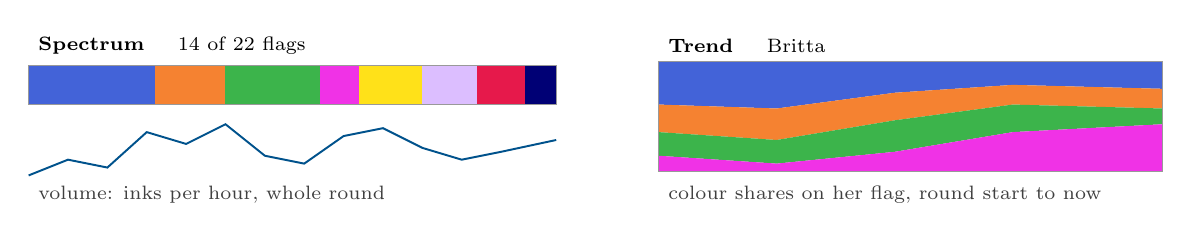
\begin{tikzpicture}[font=\scriptsize]
  % spectrum
  \node[anchor=west,font=\scriptsize\bfseries] at (0,2.35) {Spectrum \quad\normalfont 14 of 22 flags};
  \fill[ink7] (0.00,1.6) rectangle (1.60,2.1);
  \fill[ink2] (1.60,1.6) rectangle (2.50,2.1);
  \fill[ink5] (2.50,1.6) rectangle (3.70,2.1);
  \fill[ink9] (3.70,1.6) rectangle (4.20,2.1);
  \fill[ink3] (4.20,1.6) rectangle (5.00,2.1);
  \fill[ink11] (5.00,1.6) rectangle (5.70,2.1);
  \fill[ink1] (5.70,1.6) rectangle (6.30,2.1);
  \fill[ink14] (6.30,1.6) rectangle (6.70,2.1);
  \draw[black!40] (0,1.6) rectangle (6.7,2.1);
  \draw[brandskydark,line width=0.7pt] (0,0.7) -- (0.5,0.9) -- (1,0.8) -- (1.5,1.25) -- (2,1.1) -- (2.5,1.35) -- (3,0.95) -- (3.5,0.85) -- (4,1.2) -- (4.5,1.3) -- (5,1.05) -- (5.5,0.9) -- (6,1.0) -- (6.7,1.15);
  \node[anchor=west,text=muted] at (0,0.45) {volume: inks per hour, whole round};
  % trend
  \begin{scope}[xshift=8cm]
    \node[anchor=west,font=\scriptsize\bfseries] at (0,2.35) {Trend \quad\normalfont Britta};
    \fill[ink7] (0,1.6) -- (1.5,1.55) -- (3,1.75) -- (4.5,1.85) -- (6.4,1.8) -- (6.4,2.15) -- (0,2.15) -- cycle;
    \fill[ink2] (0,1.25) -- (1.5,1.15) -- (3,1.4) -- (4.5,1.6) -- (6.4,1.55) -- (6.4,1.8) -- (4.5,1.85) -- (3,1.75) -- (1.5,1.55) -- (0,1.6) -- cycle;
    \fill[ink5] (0,0.95) -- (1.5,0.85) -- (3,1.0) -- (4.5,1.25) -- (6.4,1.35) -- (6.4,1.55) -- (4.5,1.6) -- (3,1.4) -- (1.5,1.15) -- (0,1.25) -- cycle;
    \fill[ink9] (0,0.75) -- (1.5,0.75) -- (3,0.75) -- (4.5,0.75) -- (6.4,0.75) -- (6.4,1.35) -- (4.5,1.25) -- (3,1.0) -- (1.5,0.85) -- (0,0.95) -- cycle;
    \draw[black!40] (0,0.75) rectangle (6.4,2.15);
    \node[anchor=west,text=muted] at (0,0.45) {colour shares on her flag, round start to now};
  \end{scope}
\end{tikzpicture}
\caption{The two aggregate views, as sketches.}
\label{fig:aggregates}
\end{figure}

% ================================================================= 13
\section{Galleries and the play record}\label{sec:gallery}

\begin{decision}{D14}{What does F1R3Ink publish?}
\textbf{Recommendation: two kinds, linked.}
\begin{itemize}[leftmargin=1.2em,itemsep=1pt]
\item \code{round}, as the Portal already registers it: the history of a span of the round, by
  default the whole of it. Any participant may publish one, and the host is offered it at the
  close. It holds only what is already public on the chain, so publishing it discloses nothing.
  Private flags appear as their volume and their sealed events.
\item \code{flag}, a portrait: one person's flag over a span, with its history. Only the flag's
  owner may publish it. A portrait of a private flag includes the content keys of the inks it
  shows, so it discloses them, and anyone can verify them against the chain. Portraits link to
  their round with \code{linkPlays}, in both directions.
\end{itemize}
\end{decision}

\textbf{Encoding.} The \code{round} body is a byte array that rebuilds from \code{f1r3ink.log}:

\begin{lstlisting}
"F1NK"  u8 version = 1  u32 from  u32 to  u8 unit-steps  u32 unit-ms
u8 P   P x 3 bytes                  the palette
varint N  N x 20 bytes              addresses, in order of first appearance
varint A  A x 16 bytes              anonymous handles, in order of first appearance
varint E  E x (varint dh, varint dt_ms, u8 type, payload)   events in history order
   type 0 visibility   u8 player, u8 public?
   type 1 tags         u8 player, varint len, UTF-8 tags joined by U+001F
   type 2 ink          u8 target, stripe, ink
   type 3 veil         u8 player, varint n, n x stripe
   type 4 reveal       varint handle, u8 player
stripe := u8 0, u8 player  |  u8 1, varint handle
ink    := u8 0, u8 colour  |  u8 1 (lifted)
        |  u8 2, u8 colour or 255, 32-byte envelope hash
\end{lstlisting}

A sealed ink carries its colour only if its owner disclosed it within the span. The
\code{flag} body uses the same layout restricted to one target, with the content keys appended
as \code{varint K, K x (event index, 32 bytes)}. The header's \code{preview} is the frame at the
span's end: for each public flag, its stripes as colour and remaining steps. That is at most two
bytes per stripe.

A play is \emph{verifiable}. Anyone can rebuild its body from \code{log} at its recorded block,
check every disclosed key against its envelope, and compare hashes.

\textbf{Engagement.} Views and likes go through the Portal's \code{engage} and order the gallery,
as in F1R3Pix. F1R3Ink does not breed plays.

% ================================================================= 14
\section{Security and abuse}\label{sec:security}

Everything in F1R3Pix's table applies to messages and payments. The rows below are the threats
F1R3Ink adds.

\begin{center}\small
\begin{tabularx}{\linewidth}{@{}>{\raggedright\arraybackslash}p{40mm} X@{}}
\toprule
threat & answer\\
\midrule
Writing someone else's stripe & Impossible: \code{ink} writes only the caller's own stripe. Only the relay writes anonymous stripes.\\
Flooding a flag & One stripe per inker per target, and \code{minInterval} between inks (D9).\\
Hurtful inks & A colour carries no fixed meaning, and the game has no words in a flag. A target may \emph{veil} stripes on their public flag from other players' view (D15). Their colours stay on the chain, and the target always sees them. A private flag shows a target's stripes to no one else.\\
Unmasking anonymous inkers & The chain never carries the inker's address against an anonymous stripe. Timing is blurred by batching, and anonymity is refused below \code{anonMin}. The relay knows the inker (D10). A small round leaks through who was online, and the client says so.\\
A dishonest relay & It cannot forge an ink, because it holds the inker's signed request. It could drop or delay inks. Clients read their anonymous inks back and report any that never land. The Cooperative can rotate the relay key.\\
Fresh-looking stripes & Decay runs on block time, which the inker does not choose (\S\ref{sec:order}).\\
Replaying a sealed ink & The envelope's \code{aad} binds the instance, target, stripe and sequence number.\\
False disclosure & Each disclosed key is checked against its envelope, and a stripe whose key fails is drawn veiled and marked.\\
Payments for inks & Payments are public metadata, as in F1R3Pix, so payments followed by inks are visible to all. A colour has no fixed meaning to buy. The game does not forbid deals, just as F1R3Pix does not.\\
Metadata & Who inks a private flag, and when, is public for attributed stripes. Volume is public for every flag.\\
\bottomrule
\end{tabularx}
\end{center}

\begin{decision}{D15}{May a target hide stripes on their own flag?}
\textbf{Recommendation: yes, from other players' view of a public flag only, by \code{veil}.} A
public flag is a disclosure, and its owner should not have to disclose a stripe they find
hurtful in order to disclose the rest. A veiled stripe is drawn as a neutral grey bar with no
colour, so its presence stays honest. Veiling does not remove anything from the chain, and it
does not change what the owner sees. The client tells the owner both of these things.
\end{decision}

% ================================================================= 15
\section{Manifest and conformance}\label{sec:manifest}

\begin{lstlisting}
{ "id": "f1r3ink", "name": "F1R3Ink",
  "tagline": "Say how you see each other, in colour.",
  "entry": "<entry-base>/f1r3ink/", "platforms": ["web"],
  "env": "rho:id:...",                       // unchanged URI; environment version raised
  "templates": [ "f1r3ink.enter", "f1r3ink.tags", "f1r3ink.visibility",
                 "f1r3ink.ink", "f1r3ink.veil", "f1r3ink.say",          // play
                 "f1r3ink.players", "f1r3ink.flags", "f1r3ink.history",
                 "f1r3ink.log", "f1r3ink.mail", "f1r3ink.outbox" ],      // explore
  "capabilities": ["pay", "open", "relay"],
  "relay": "<relay-base>/f1r3ink/",
  "galleries": [
      { "kind": "round", "renderer": "<entry-base>/f1r3ink/preview/round.html" },
      { "kind": "flag",  "renderer": "<entry-base>/f1r3ink/preview/flag.html" } ],
  "contactsDialogue": true, "readerTier": false, "minProtocol": 2 }
\end{lstlisting}

The installed template \code{f1r3ink.state} is retired. \code{relayInk}, \code{relayReveal} and
\code{setRelay} are not game templates: they are signed only by the relay key or the registry
key, and are absent from the manifest.

\textbf{Conformance tests} extend the Portal's, F1R3Pix's and F1R3Beat's:

\begin{itemize}[leftmargin=1.2em,itemsep=1pt]
\item the environment and every template parse with the node's own parser and normalise with
  its compiler, as the F1R3Beat work found necessary. Every play template binds no deployer
  authority;
\item decay vectors: for a set of stripes and times, the Rust and TypeScript opacity functions
  agree, including at every step boundary and at the close;
\item sealed inks seal in TypeScript and open in the Rust wallet with unlabelled wraps, refuse
  to open under another game, instance, stripe or sequence number, and verify under a
  disclosed key;
\item relay handles: given a secret and inputs, the relay's handle matches the vector, and a
  signed request with a wrong domain is refused;
\item the \code{round} and \code{flag} encodings round-trip against shared vectors in Rust and
  TypeScript;
\item end to end against the mock node: enter, tag, ink attributed and anonymous, refresh, lift,
  switch visibility with disclosure, veil, say, open, pay, close, and publish a round and a
  portrait that both rebuild from the chain.
\end{itemize}

% ================================================================= 16
\section{F1R3Gaze}\label{sec:gaze}

F1R3Ink needs the \code{pay} and \code{open} rows that F1R3Pix adds to the Portal's
\code{GAZE-MAPPING.md}, with \code{open} extended to unlabelled wraps. It adds one capability:
\code{relay}, a signature under a fixed domain, bound to one URL named in the game's manifest,
which never yields the key and cannot be pointed elsewhere. Like \code{open}, it is a wallet
operation with a caller-fixed purpose. That is the shape F1R3Gaze's wallet capabilities already
take. \code{GAZE-MAPPING.md} should gain the row when Phase~2 lands.

% ================================================================= 17
\section{Development plan}\label{sec:plan}

\begin{center}\small
\begin{tabularx}{\linewidth}{@{}>{\raggedright\arraybackslash}p{28mm} X >{\raggedright\arraybackslash}p{44mm}@{}}
\toprule
phase & work & done when\\
\midrule
1 · Environment & New \code{f1r3ink.rho} body: \code{enter}, \code{tags}, \code{visibility}, \code{ink}, \code{veil}, \code{say}, the relay moves and \code{setRelay}; reads; configuration; decay and encoding vectors. & Parses and normalises; template rules pass; mock-node tests of every move and read.\\
2 · Sealing and relay & Ink envelope with unlabelled wraps in TypeScript and the Rust wallet; \code{open} extended; host \code{relay}; the relay as a service beside \code{f1r3games-service}; \code{statusAt} in the Portal. & Seal, open and disclose vectors pass; an anonymous ink lands from a signed request.\\
3 · Client & Core and views: flags, wheel, ink control, history popover, tags, visibility; messages and tokens from the F1R3Pix core; spectrum and trend; accessibility; tabs. & A full round against the mock node with six simulated players, public and private, attributed and anonymous.\\
4 · Live shard & Install on an ign1t10n shard; measure phlo for each move, the \code{flags} read at 24 and 64 participants, and the relay's window. & One live round of at least eight players, start to close, with decay visibly at work.\\
5 · Galleries & \code{round} and \code{flag} encodings, publishing, renderers, engagement. & A closed round publishes both kinds, and both rebuild and verify from the chain.\\
Later & Trustless anonymity; replies to anonymous stripes; disclosure stipends; partial disclosure; tournaments; the F1R3Gaze version. & \\
\bottomrule
\end{tabularx}
\end{center}

Phases 1 and 2 can proceed together, and Phase~3 can begin against stubs. The client reuses
F1R3Pix's core for messages, payments and the wheel, and F1R3Beat's pattern for reading the
gallery from inside the game.

% ================================================================= 18
\section{Decisions}\label{sec:decisions}

\begin{center}\small
\begin{tabularx}{\linewidth}{@{}l>{\raggedright\arraybackslash}p{38mm}X@{}}
\toprule
 & question & decision or recommendation\\
\midrule
D1 & \textbf{Settled.} Flag visibility & Public or private per player; public flags seen in full by everyone. \emph{Recommended:} private inks sealed to owner and inker; going public discloses current colours; no preselected default.\\
D2 & \textbf{Settled.} Attribution & Declared by the inker. \emph{Recommended:} per stripe, at first ink; attributed by default; anonymous via the relay; reveal one way; \code{anonMin} 5.\\
D3 & \textbf{Settled.} Re-inking & One mutable stripe per inker per target, with its history on right-click. \emph{Recommended:} same colour refreshes; lifting allowed.\\
D4 & \textbf{Settled.} Colour & A palette. \emph{Recommended:} host-chosen, 2--32 colours, default sixteen; identified by number, never by name.\\
D5 & \textbf{Settled.} Decay & Opacity falls per unit until refreshed or gone. \emph{Recommended:} $1/k$ per unit $u$ on block time; presets, default one hour by 24; faded stripes keep their place.\\
D6 & Phases & Lobby: enter, tags, visibility, talk, pay. Active: also ink. Closed: read only.\\
D7 & Round size & Capacity fixed at creation, 3--64, default 24; leavers keep the stripes they gave.\\
D8 & Rewarding disclosure & The commons, the portrait and the conversation; show-to-see as a host option, off by default; a disclosure stipend later.\\
D9 & Pacing & One ink per stripe per minute of block time; client coalescing.\\
D10 & Trust in the relay & A trusted relay run by the Cooperative in version 1, said plainly in the client.\\
D11 & \textbf{Settled.} Messages and payments & Included, exactly as F1R3Pix and F1R3Beat.\\
D12 & Wheel order & Most recent interaction first; by name, or newest stripe on you, on request.\\
D13 & \textbf{Settled.} Aggregates & Spectrum and trend, chosen by the player. \emph{Recommended:} built only from what the viewer may see; volume counts every ink.\\
D14 & Galleries & \code{round} (anyone, public data only) and \code{flag} (owner only), linked and verifiable.\\
D15 & Veiling & An owner may veil stripes from others' view of a public flag.\\
\bottomrule
\end{tabularx}
\end{center}

The author of the game also settled the visibility rule of \S\ref{sec:visibility}. It is not
set out as a decision of its own, because D1 and D8 rest on it.

\subsection{Out of scope for version 1}\label{sec:future}

Trustless anonymity through anonymous credentials, once F1R3Node-Rust offers ring signatures,
blind signatures or zero-knowledge membership proofs as system processes; replies from a target
to an anonymous inker through the relay; disclosure stipends through sponsorships; partial
disclosure, a flag public to chosen players only; tags private to some players; correlating
sentiment across games; tournaments; hidden recipient lists and a report flow, as in F1R3Pix;
and the F1R3Gaze version.

\end{document}
